








%%%%%%%%%%%%%%%%%%%%%%%%%%%%%%%%%%%%%%%%%
% Beamer Presentation
% LaTeX Template
% Version 1.0 (10/11/12)
%
% This template has been downloaded from:
% http://www.LaTeXTemplates.com
%
% License:
% CC BY-NC-SA 3.0 (http://creativecommons.org/licenses/by-nc-sa/3.0/)
%
%%%%%%%%%%%%%%%%%%%%%%%%%%%%%%%%%%%%%%%%%

%----------------------------------------------------------------------------------------
%	PACKAGES AND THEMES
%----------------------------------------------------------------------------------------

\documentclass{beamer}

\mode<presentation> {

% The Beamer class comes with a number of default slide themes
% which change the colors and layouts of slides. Below this is a list
% of all the themes, uncomment each in turn to see what they look like.

%\usetheme{default}
%\usetheme{AnnArbor}
%\usetheme{Antibes}
%\usetheme{Bergen}
%\usetheme{Berkeley}
%\usetheme{Berlin}
%\usetheme{Boadilla}
%\usetheme{CambridgeUS}
%\usetheme{Copenhagen}
%\usetheme{Darmstadt}
%\usetheme{Dresden}
%\usetheme{Frankfurt}
%\usetheme{Goettingen}
%\usetheme{Hannover}
%\usetheme{Ilmenau}
%\usetheme{JuanLesPins}
%\usetheme{Luebeck}
\usetheme{Madrid}
%\usetheme{Malmoe}
%\usetheme{Marburg}
%\usetheme{Montpellier}
%\usetheme{PaloAlto}
%\usetheme{Pittsburgh}
%\usetheme{Rochester}
%\usetheme{Singapore}
%\usetheme{Szeged}
%\usetheme{Warsaw}

% As well as themes, the Beamer class has a number of color themes
% for any slide theme. Uncomment each of these in turn to see how it
% changes the colors of your current slide theme.

%\usecolortheme{albatross}
%\usecolortheme{beaver}
%\usecolortheme{beetle}
%\usecolortheme{crane}
%\usecolortheme{dolphin}
%\usecolortheme{dove}
%\usecolortheme{fly}
%\usecolortheme{lily}
%\usecolortheme{orchid}
%\usecolortheme{rose}
%\usecolortheme{seagull}
%\usecolortheme{seahorse}
%\usecolortheme{whale}
%\usecolortheme{wolverine}

%\setbeamertemplate{footline} % To remove the footer line in all slides uncomment this line
%\setbeamertemplate{footline}[page number] % To replace the footer line in all slides with a simple slide count uncomment this line

%\setbeamertemplate{navigation symbols}{} % To remove the navigation symbols from the bottom of all slides uncomment this line
}

\usepackage{multicol}
\usepackage[utf8]{inputenc}
\usepackage[russian]{babel}
\usepackage{cmap}


\usepackage{verbatim}
\usepackage{fancybox}
\usepackage{ulem}
\usepackage{tikz}
\usetikzlibrary{positioning}
\usepackage{scalefnt}
\usetikzlibrary{arrows,shapes,positioning,shadows,trees,calc,backgrounds,fit,positioning}

\usepackage{graphicx} % Allows including images
\usepackage{booktabs} % Allows the use of \toprule, \midrule and \bottomrule in tables
\usepackage{textcomp}
\usepackage{listings}
\usepackage{color}
\usepackage{xcolor}
\usepackage{changepage}

\definecolor{mygreen}{rgb}{0,0.6,0}
\definecolor{mygray}{rgb}{0.5,0.5,0.5}
\definecolor{mymauve}{rgb}{0.58,0,0.82}

\lstset{ %
  backgroundcolor=\color{white},   % choose the background color; you must add \usepackage{color} or \usepackage{xcolor}
  basicstyle=\footnotesize,        % the size of the fonts that are used for the code
  breakatwhitespace=false,         % sets if automatic breaks should only happen at whitespace
  breaklines=true,                 % sets automatic line breaking
  captionpos=b,                    % sets the caption-position to bottom
  commentstyle=\color{mygreen},    % comment style
  deletekeywords={...},            % if you want to delete keywords from the given language
  escapeinside={\%*}{*)},          % if you want to add LaTeX within your code
  extendedchars=true,              % lets you use non-ASCII characters; for 8-bits encodings only, does not work with UTF-8
  frame=single,                    % adds a frame around the code
  keepspaces=true,                 % keeps spaces in text, useful for keeping indentation of code (possibly needs columns=flexible)
  keywordstyle=\color{blue},       % keyword style
  language=Octave,                 % the language of the code
  morekeywords={*,...},            % if you want to add more keywords to the set
  numbers=left,                    % where to put the line-numbers; possible values are (none, left, right)
  numbersep=5pt,                   % how far the line-numbers are from the code
  numberstyle=\tiny\color{mygray}, % the style that is used for the line-numbers
  rulecolor=\color{black},         % if not set, the frame-color may be changed on line-breaks within not-black text (e.g. comments (green here))
  showspaces=false,                % show spaces everywhere adding particular underscores; it overrides 'showstringspaces'
  showstringspaces=false,          % underline spaces within strings only
  showtabs=true,                  % show tabs within strings adding particular underscores
  stepnumber=1,                    % the step between two line-numbers. If it's 1, each line will be numbered
  stringstyle=\color{mymauve},     % string literal style
  tabsize=4,                       % sets default tabsize to 2 spaces
  %title=\lstname                   % show the filename of files included with \lstinputlisting; also try caption instead of title
}

\graphicspath{{./figures/}}

%----------------------------------------------------------------------------------------
%	TITLE PAGE
%----------------------------------------------------------------------------------------

\title[Обработка и исполнение запросов: лекция 12]{Многомерное Индексирование (Лекция 12) \\~\\ Многомерное (и не только) индексирование\\~\\ v5} % The short title appears at the bottom of every slide, the full title is only on the title page

\author{Георгий Чернышев} % Your name
\institute[ВШЭ] % Your institution as it will appear on the bottom of every slide, may be shorthand to save space
{
Высшая Школа Экономики \\ % Your institution for the title page
\medskip
\textit{chernishev@gmail.com} % Your email address
}
%\date{\today} % Date, can be changed to a custom date
\date{9 ноября 2020 г.}

\begin{document}

\begin{frame}
\titlepage % Print the title page as the first slide
\end{frame}

\begin{comment}
\begin{frame}
\frametitle{Overview} % Table of contents slide, comment this block out to remove it
\tableofcontents % Throughout your presentation, if you choose to use \section{} and \subsection{} commands, these will automatically be printed on this slide as an overview of your presentation
\end{frame}
\end{comment}

\begin{frame}
\frametitle{План}

\begin{enumerate}
  \setlength\itemsep{1em}
  \item Индексирование.
  \item Одномерное индексирование: B+-дерево.
  \item Многомерное индексирование
  \begin{itemize}
    \item Введение
    \item Запросы    
    \item Двухшаговая схема
    \item R-дерево
  \end{itemize}
  \item Методы разделения пространства на примере KD дерева
  \item Locality-Sensitive Hashing
  \item Машинное обучение и деревья
\end{enumerate}
\end{frame}

\begin{frame}
\frametitle{Индекс}

Способ ускорения доступа к данным, обычно какое-то упорядочивание.
\begin{itemize}
  \setlength\itemsep{1em}
  \item Используются древовидные структуры $B^{+}$-tree, $R$-tree;
  \item Не всегда выгодно использовать: занимает место и может ухудшить общую производительность на обновлениях; 
  \item Выбор атрибута (-ов) для индексирования отдается на откуп администратору СУБД;
  \item Существует много концептуально разных типов индексов.
\end{itemize}
\end{frame}

\begin{frame}
\frametitle{$B^{+}$-tree (1)}

Это вариант $B$-tree, отличия:

\begin{itemize}
  \setlength\itemsep{1em}
  \item Все ключи в листьях;
  \item Листья прошиты для итерирования по данным;
  \item Все уровни кроме листового должны (хорошо было бы) чтобы помещались в оперативную память.
\end{itemize}
Используются во всех индустриальных (и большинстве игрушечных) СУБД.
\end{frame}

\begin{frame}
\frametitle{$B^{+}$-tree (2): пример}

\begin{figure}[htb]
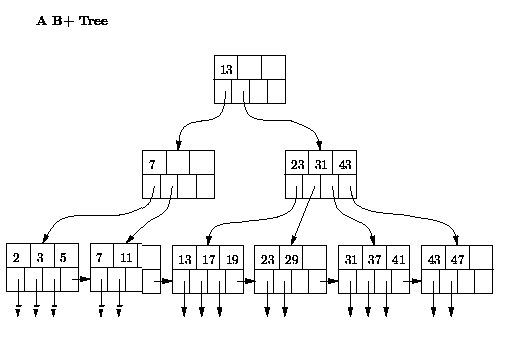
\includegraphics[width=\textwidth,height=0.75\textheight,keepaspectratio]{B-tree.png}\footnote{\tiny{Изображение взято с http://infolab.stanford.edu/~ullman/dbsi/win98/hw2.html}}
\end{figure}

\end{frame}

\begin{frame}
\frametitle{О реализации}
\begin{itemize}
  \setlength\itemsep{1em}
  \item На самом деле она очень сложна!
  \item Надо думать о физическом представлении, тюнингу под кеш-память, параллельном доступе, восстановлении и прочей интеграции с другими подсистемами СУБД.
  \item Пример: достаточно игрушечный индекс на $B^{+}$-tree это около 50 килобайт кода.
\end{itemize}
\end{frame}

\begin{frame}
\frametitle{Многомерное индексирование}

Индексирование N-мерном пространстве:
\begin{itemize}
  \setlength\itemsep{1em}
  \item Что индексируем:
  \begin{itemize}
    \item Точки;
    \item Объекты.
  \end{itemize}
  \item Для чего индексируем:
  \begin{itemize}
    \item СУБД;
    \item GIS-системы (их, кажется, побольше будет).
  \end{itemize}  
\end{itemize}
\end{frame}

\begin{frame}
\frametitle{Запросы}

Индекс разрабатывется под запросы \cite{Manolopoulos2005}:
\begin{itemize}
	\item Запрос на диапазон;
	\item Топологические запросы;
	\begin{figure}[htb]
		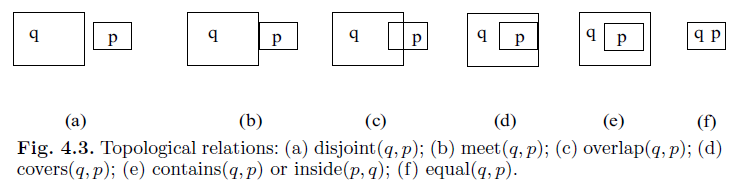
\includegraphics[width=\textwidth,height=0.3\textheight,keepaspectratio]{top-rels.png} 
		\footnote{\tiny{Изображение взято из \cite{Manolopoulos2005}}}
	\end{figure}      
	\item Запросы на направление;
	\item Запросы к ближайшим соседям (разные варианты: прямые, обратные, условные и т.д.);
	\item Запросы с пространственным соединением: многопроходные, с пространственным предикатом.
\end{itemize}
\end{frame}


\begin{frame}
\frametitle{Как индексировать объекты? Двухшаговая схема!}

Описываем объекты с помощью MBR (min. bounding rectangle).\\~\\

При поиске используем двухшаговую схему:
\begin{itemize}
	\item Фильтрация, получение списка кандидатов;
	\item Проверка списка кандидатов, очистка от ложных срабатываний.
\end{itemize}


\begin{figure}[htb]
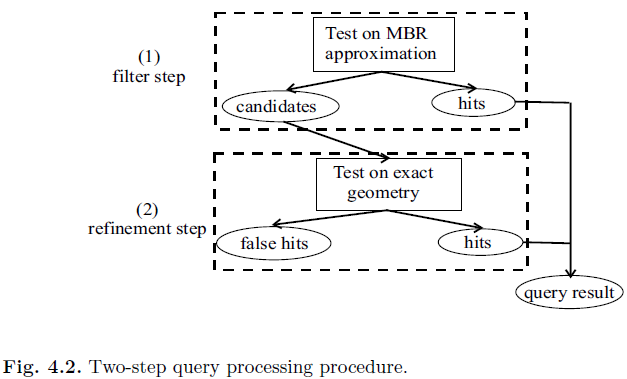
\includegraphics[width=\textwidth,height=0.55\textheight,keepaspectratio]{2step.png} 
\footnote{\tiny{Изображение взято из \cite{Manolopoulos2005}}}
\end{figure}   

\end{frame}

\begin{frame}
\frametitle{$R$-tree (1)}
\begin{itemize}
  \setlength\itemsep{1em}
  \item Древовидная структура для упрощения поиска;
  \item Можно сказать что это обобщение $B^{+}$-tree на многомерный случай;
  \item Используется в индустриальных СУБД и GIS системах: PostgreSQL, Oracle, SQLite, PostGIS, MapInfo, ... 
  \begin{itemize}
    \item фактически индустриальный стандарт для многомерных данных малой размерности;
  \end{itemize}
  \item Есть в Boost и куче других приложений, вне СУБД.
\end{itemize}

\end{frame}


\begin{frame}
\frametitle{$R$-tree (2): популярность}

\begin{figure}[htb]
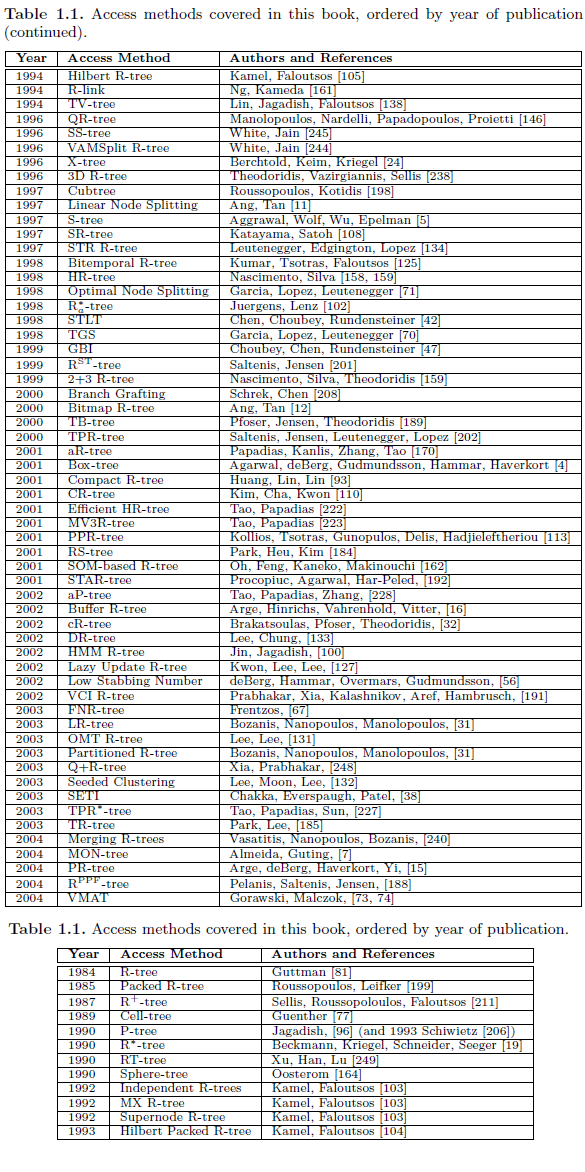
\includegraphics[width=\textwidth,height=0.8\textheight,keepaspectratio]{r-tree-works.png} 
\footnote{\tiny{Изображение взято из \cite{Manolopoulos2005}}}
\end{figure}   

\end{frame}


\begin{frame}
\frametitle{$R$-tree (3): определение}

Согласно  \cite{Manolopoulos2005} R-дерево~--- это древовидная структура данных, заданная парой $(m, M)$ со следующими свойствами:

\begin{itemize}
  \setlength\itemsep{1em}
  \item Каждый лист может содержать до $M$ записей, минимально $2 \le m \le M / 2$.
  \item Каждая запись в листе представлена в форме (mbr, oid), где mbr это минимальный ограничивающий прямоугольник, а oid~--- идентификатор объекта.
  \item Количество записей хранящихся во внутреннем узле также должно при-
надлежать $[m; M]$. Каждая запись в узле представляет собой пару (mbr,
p), где p — указатель на ребенка узла, а mbr содержит в себе mbr ребенка.
  \item Дерево сбалансировано~--- все листья находятся на одном уровне.
\end{itemize}

\end{frame}



\begin{frame}
\frametitle{$R$-tree (4): пример}

\begin{figure}[htb]
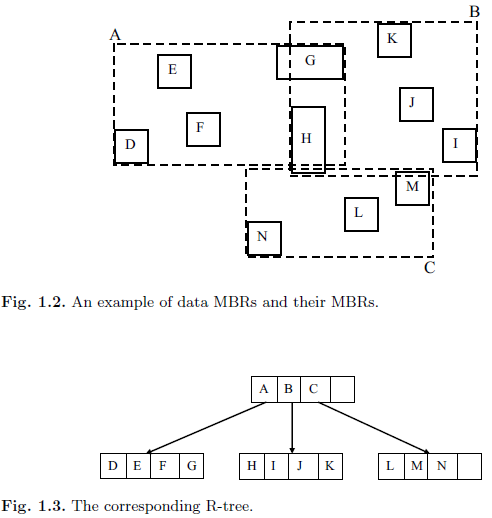
\includegraphics[width=\textwidth,height=0.8\textheight,keepaspectratio]{example.png} 
\footnote{\tiny{Изображение взято из \cite{Manolopoulos2005}}}
\end{figure}   

\end{frame}

\begin{frame}
\frametitle{$R$-tree (5): свойства}
\begin{itemize}
  \setlength\itemsep{1em}
  \item Теперь у нас не диапазоны, а ``коробочки''~--- многомерные прямоугольники;
  \item Сложно расщеплять вершину: $NP$-трудная задача + много критериев;
  \item Сложно искать, $MBR$ могут пересекаться $\rightarrow$ надо проверить много путей до листьев;
\end{itemize}

\end{frame}

\begin{frame}
\frametitle{Вычисление диапазонного запроса}

\begin{figure}[htb]
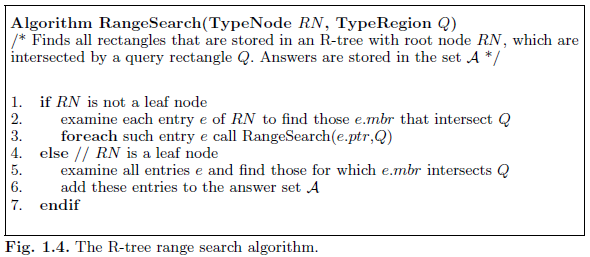
\includegraphics[width=\textwidth,height=0.8\textheight,keepaspectratio]{range.png} 
\footnote{\tiny{Изображение взято из \cite{Manolopoulos2005}}}
\end{figure}   

\end{frame}

\begin{frame}
\frametitle{Вставка в $R$-tree I}

\begin{figure}[htb]
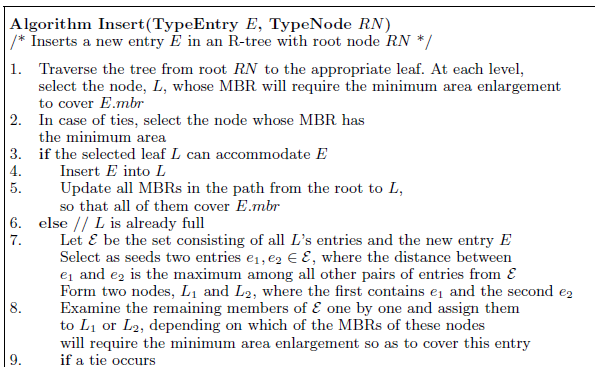
\includegraphics[width=\textwidth,height=0.8\textheight,keepaspectratio]{insert3.png} 
\footnote{\tiny{Изображение взято из \cite{Manolopoulos2005}}}
\end{figure}   

\end{frame}

\begin{frame}
\frametitle{Вставка в $R$-tree II}

\begin{figure}[htb]
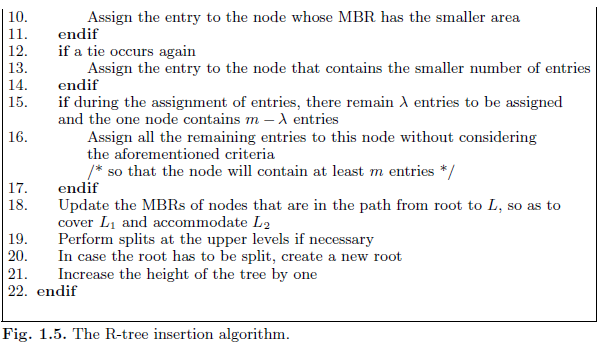
\includegraphics[width=\textwidth,height=0.8\textheight,keepaspectratio]{insert4.png} 
\footnote{\tiny{Изображение взято из \cite{Manolopoulos2005}}}
\end{figure}   

\end{frame}

\begin{frame}
\frametitle{Задача расщепления вершины}

Строки 6--17 на самом деле отдельный алгоритм.

\begin{itemize}
  \setlength\itemsep{1em}
  \item Много критериев: суммарная площадь, периметр, пересечение и т.д.
  \begin{figure}[htb]
  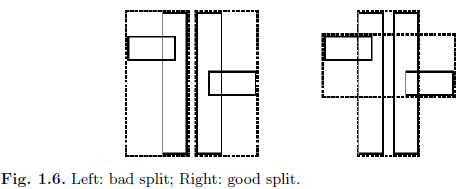
\includegraphics[width=\textwidth,height=0.2\textheight,keepaspectratio]{delete.png} 
  \footnote{\tiny{Изображение взято из \cite{Manolopoulos2005}}}
  \end{figure}   
  \item $NP$-трудная задача, доказано;
  \item А значит и много подходов к решению: Al-Badarneh's et al. split, Corner-Based split, K-means split, Hilbert split, $RR^*$ split, $R^*$ split, Greenes split, Guttman Quadratic and Linear splits, Ang and Tan split, Double-Sorting Based split.
\end{itemize}

\end{frame}

\begin{frame}
\frametitle{Применение K-means}

  \begin{figure}[htb]
  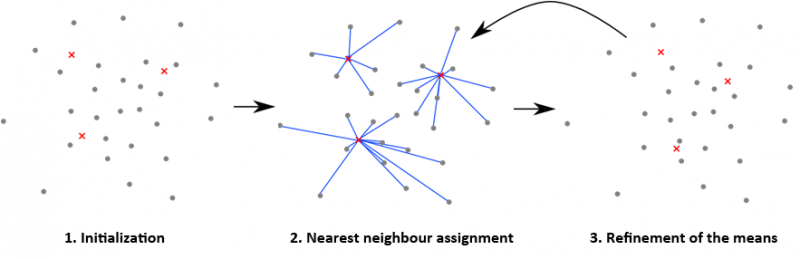
\includegraphics[width=\textwidth,height=0.4\textheight,keepaspectratio]{steps-of-kmeans.png} 
  \footnote{\tiny{Изображение взято из \url{https://prateekvjoshi.com/2013/06/06/what-is-k-means-clustering/}}}
  \end{figure}   

\begin{itemize}
  %\setlength\itemsep{1em}
  \item Исходная работа \cite{Brakatsoulas2002}
  \item Проблема~--- для сходимости в случае прямоугольников нужно либо доказывать ее, либо нужны: 
  \begin{enumerate}
    \item правильная метрика расстояния между многоугольниками;
    \item правильная формула центроида.
  \end{enumerate}
  \item Математически обоснованное решение \cite{Grigorev2016};
\end{itemize}

\end{frame}

\begin{frame}
\frametitle{$R$-tree: варианты}

Основные варианты \cite{Papadopoulos2009}:

\begin{itemize}
  \setlength\itemsep{1em}
  \item $R^*$~--- повторная вставка при расщеплении;
  \item $R^+$~--- объект может покрываться несколькими mbr;
  \item Гильбертово R-дерево~--- учет точки на гильбертовой кривой;
  \item Есть более 70 вариантов;
\end{itemize}

\end{frame}

\begin{frame}
\frametitle{Что бывает еще?}

Классификация:

\begin{itemize}
  \setlength\itemsep{1em}
  \item Методы выделения пространства~--- $R$-tree, $RD$-tree $SR$-tree;
  \item Методы разделения пространства~--- quadtree, $Kd$-tree, tries;
\end{itemize}

Реализация в постгрес (обобщенная модель с транзакционностью):
\begin{itemize}
  \setlength\itemsep{1em}
  \item GiST\footnote{http://www.sai.msu.su/~megera/postgres/gist/};
  \item SP-GiST\footnote{https://www.postgresql.org/docs/9.2/static/spgist-intro.html} \cite{Eltabakh2006};
\end{itemize}


\end{frame}

\begin{frame}
\frametitle{$Kd$-дерево}
Суть:
\begin{itemize}
  \setlength\itemsep{1em}
  \item Имея $n$-мерный набор точек расщепляем его последовательно по $x_1$, $x_2$, $\ldots$ $x_n$, $x_1$, $x_2$, $\ldots$;
  \item На $i$-м шаге расщепления делим наш набор по медиане $i$-ой координаты на две части, ``проводим'' черту разбивающая наше пространство на две части;
  \item На $i+1$-м шаге аналогично поступаем с каждой половиной точек оставшейся от $i$-го.
  
\end{itemize}

\end{frame}

\begin{frame}
\frametitle{Двумерный пример}

\begin{figure}[htb]
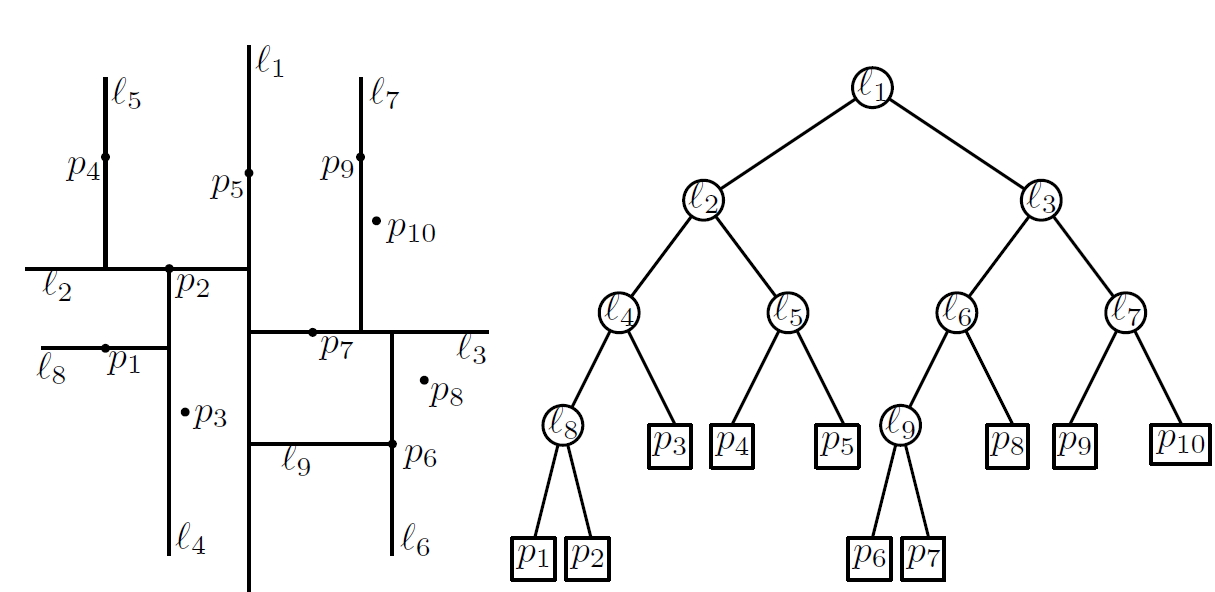
\includegraphics[width=\textwidth,height=0.8\textheight,keepaspectratio]{ex1.png} 
\footnote{\tiny{Изображение взято из \url{https://www.cise.ufl.edu/class/cot5520fa09/CG_RangeKDtrees.pdf}}}
\end{figure}   

\end{frame}

\begin{frame}
\frametitle{Как строить}

\begin{figure}[htb]
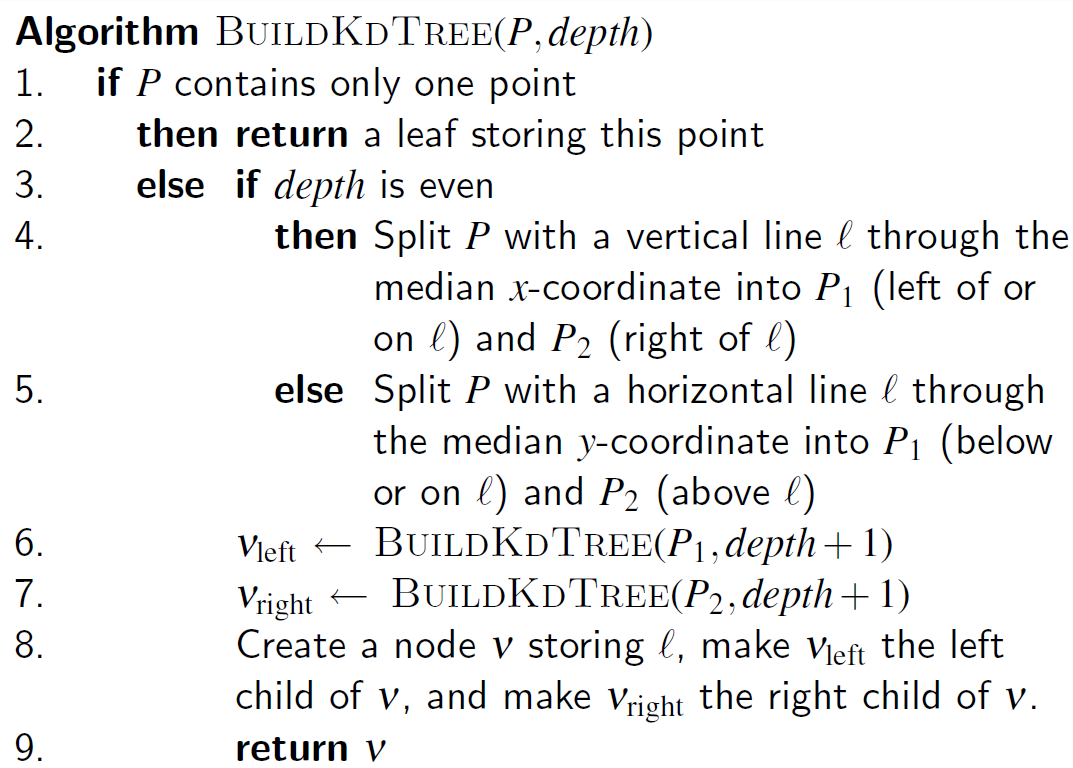
\includegraphics[width=\textwidth,height=0.8\textheight,keepaspectratio]{ex2.png} 
\footnote{\tiny{Изображение взято из \url{https://www.cise.ufl.edu/class/cot5520fa09/CG_RangeKDtrees.pdf}}}
\end{figure}   

\end{frame}

\begin{frame}
\frametitle{Запросы}

Регион либо хранится с каждым узлом, либо вычисляется налету.

\begin{figure}[htb]
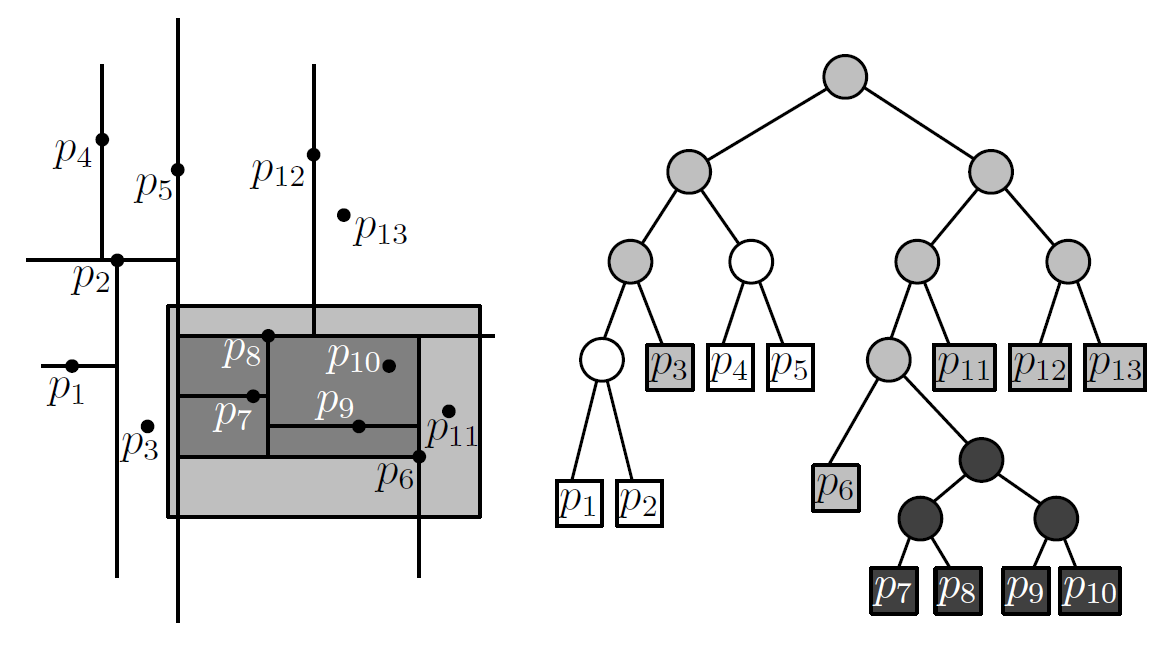
\includegraphics[width=\textwidth,height=0.7\textheight,keepaspectratio]{ex3.png} 
\footnote{\tiny{Изображение взято из \url{https://www.cise.ufl.edu/class/cot5520fa09/CG_RangeKDtrees.pdf}}}
\end{figure}   

\end{frame}

\begin{frame}
\frametitle{Как на практике обстоят дела с деревьями?}

\begin{itemize}
  \setlength\itemsep{1em}
  \item С ростом размерности очень сильно растет время построения и время исполнения запросов.
  \item Что происходит? Приходится проверять всё больший и больший \% индекса~--- \alert{curse of dimensionality};
  \item Например, в 8-ми мерном пространстве поиск может быть в 16 раз медленнее чем в двумерном на индексе с $R$-tree;
  \item Понижение размерности~--- PCA, SVD и прочее~--- не помогает;
  \item \alert{Математики доказали что это неизбежно для деревьев};
\end{itemize}

Поэтому, область применения деревьев~--- $R$-tree до 10 измерений, отдельные варианты до 30-40 ($RR^*$-tree). В тоже время, индустрии нужны десятки-сотни тысяч...

\end{frame}


\begin{frame}
\frametitle{Что делать?}

Locality-Sensitive Hashing (LSH) \cite{Gionis1999}, суть:

\begin{itemize}
  \setlength\itemsep{1em}
  \item Имеем набор хеш-функций, они распределяют объекты по ведрам;
  \item Хеш-функции заданы так, чтобы вероятность коллизии была была максимальна если объекты близки. 
\end{itemize}

Увы:

\begin{itemize}
  \setlength\itemsep{1em}
  \item Работает только для kNN, дубликатов и еще некоторых типов;
  \item Не точно: не только возвращает то, что не годится, \\ но вдобавок еще и ``теряет'' нужные данные!
  \item Впрочем, есть оценки насколько неточно. 
\end{itemize}

Вроде как, работает на практике.

\end{frame}

\begin{frame}
\frametitle{Что еще бывает из деревьев?}
\scriptsize
\begin{multicols}{2}
\begin{itemize}
	\setlength\itemsep{1em}
	\item M-tree \cite{Ciaccia1997}~--- дерево для запросов по подобию с произвольной метрикой;
	\item ND-tree \cite{Qian2006}~--- дерево для индексирования неупорядоченных дискретных многомерных значений, например генетических последовательностей.
	\item VP-tree \cite{Yianilos1993}~--- в метрическом пространстве выбираем точку и делим данные на те, что ближе трешолда и те что дальше.
	\item ...
	
\end{itemize}

Кто хочет еще больше деревьев~--- смотрите книжку Hanan Samet'а.

	\columnbreak
	
\begin{figure}[htb]
	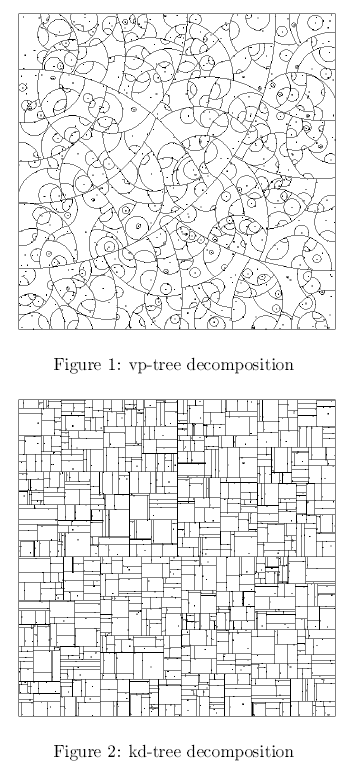
\includegraphics[width=\textwidth,height=0.8\textheight,keepaspectratio]{vp-tree.png} 
	\footnote{\tiny{Изображение взято из \cite{Yianilos1993}}}
\end{figure}

\end{multicols}

\end{frame}

\begin{frame}
	\frametitle{Деревья в 202* году}
	
	Кажется c перспективами деревьев всё довольно плохо, есть вероятность что в ближайшие годы они очень сильно потеряют в значимости. А может даже будут просто убраны из вводного курса информатики!\\~\\
	
	Что случилось? Машинное обучение наступает :(\\~\\
	
	J. Ding et al. 2020. ALEX: An Updatable Adaptive Learned Index. In Proceedings of the 2020 ACM SIGMOD International Conference on Management of Data (SIGMOD '20). Association for Computing Machinery, New York, NY, USA, 969–984.
	
\end{frame}

\begin{frame}
	\frametitle{ALEX: идея}
	\begin{figure}[htb]
		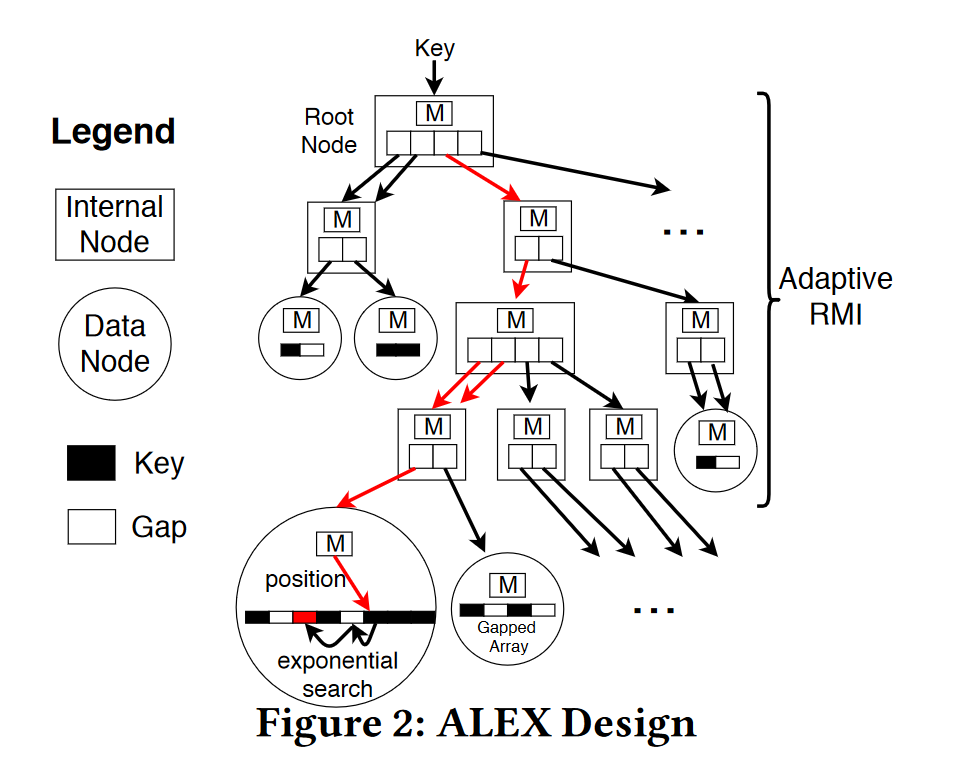
\includegraphics[width=\textwidth,height=0.8\textheight,keepaspectratio]{alex-design.png} 
		\footnote{\tiny{Изображение взято с архивной версии соответствующей статьи}}
	\end{figure}	
	
\end{frame}

\begin{frame}
	\frametitle{ALEX: бенчмарк}
	% общая производительность	
	\begin{figure}[htb]
	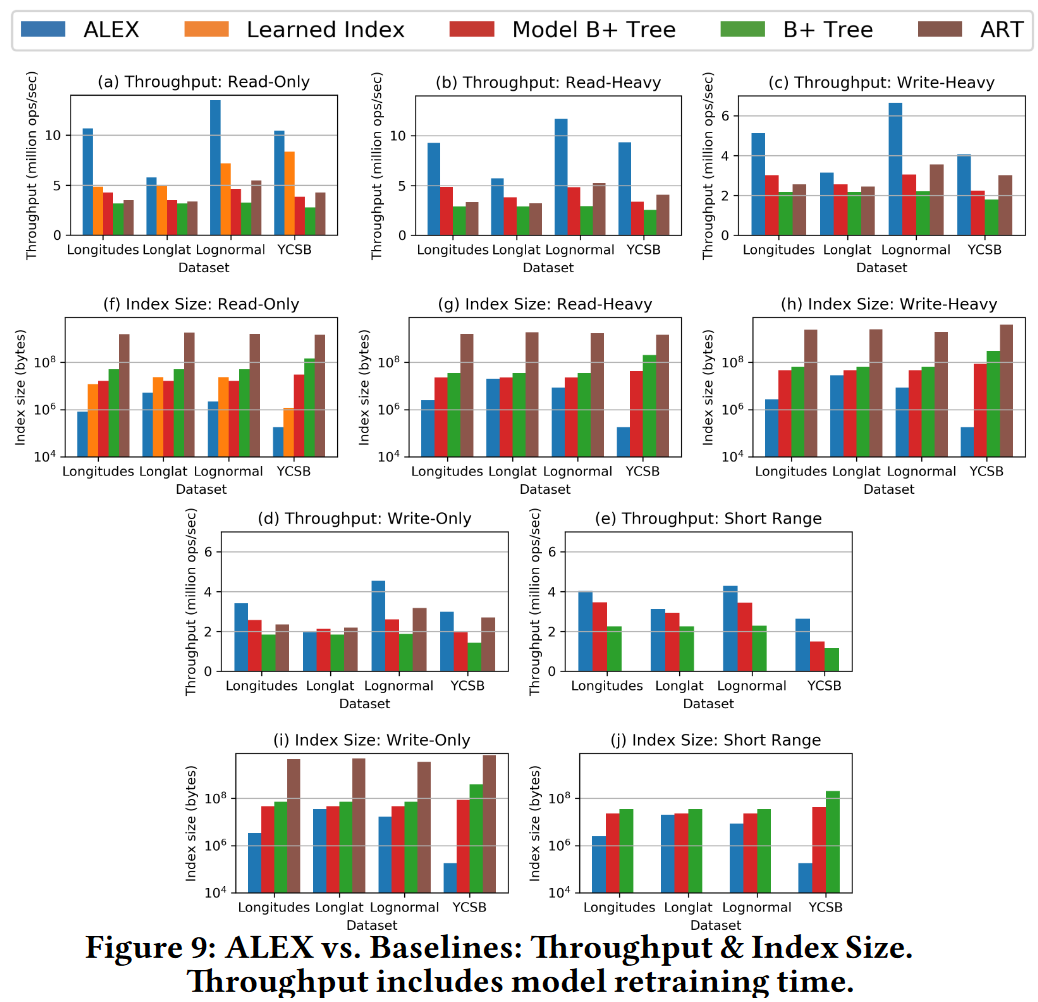
\includegraphics[width=\textwidth,height=0.8\textheight,keepaspectratio]{alex-bench-1.png} 
	\footnote{\tiny{Изображение взято с архивной версии соответствующей статьи}}
	\end{figure}	
\end{frame}

\begin{frame}
	\frametitle{ALEX: бенчмарк II}
	% ошибки	
	\begin{figure}[htb]
	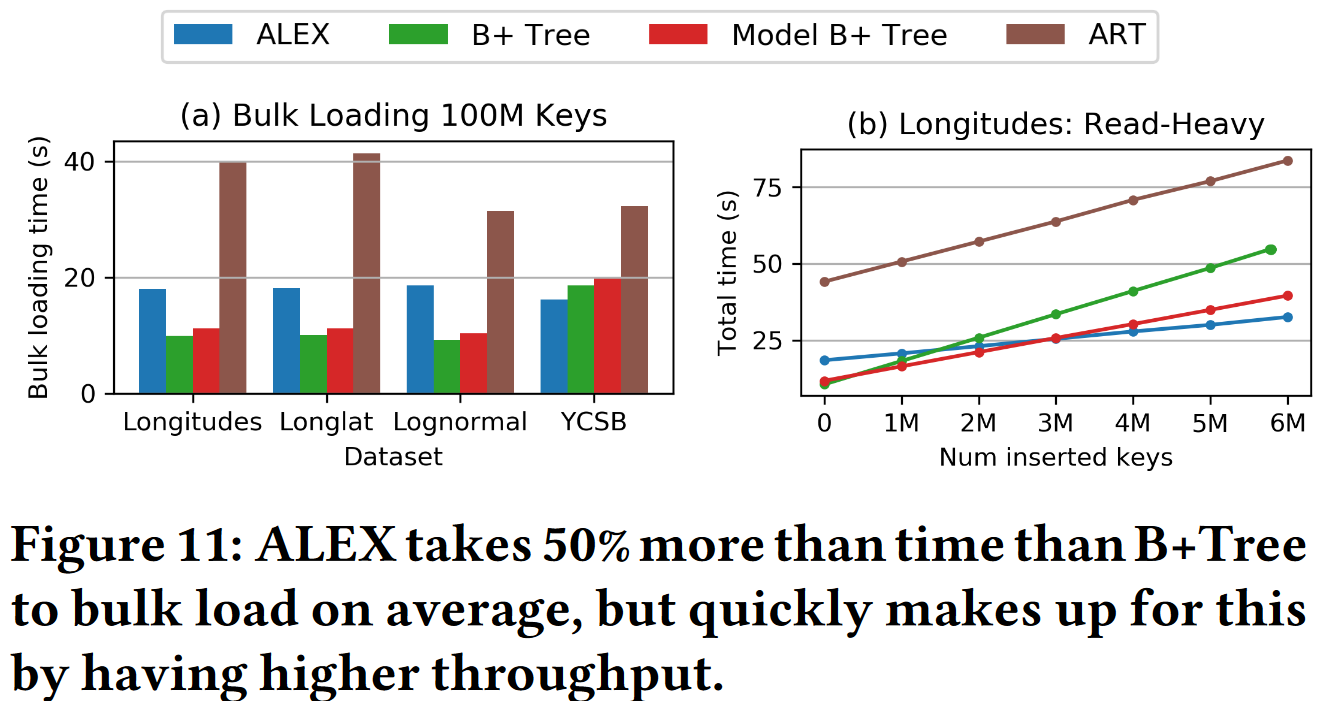
\includegraphics[width=\textwidth,height=0.8\textheight,keepaspectratio]{alex-bench-2.png} 
	\footnote{\tiny{Изображение взято с архивной версии соответствующей статьи}}
\end{figure}	
	

	
\end{frame}


\begin{frame}
	\frametitle{А что с многомерностью?}


Z. Yang et al. 2020. Qd-tree: Learning Data Layouts for Big Data Analytics. In Proceedings of the 2020 ACM SIGMOD International Conference on Management of Data (SIGMOD '20). Association for Computing Machinery, New York, NY, USA, 193–208. 


\end{frame}


\begin{comment}
\begin{frame}[t]
\frametitle{Примеры систем}

\begin{figure}[htb]
%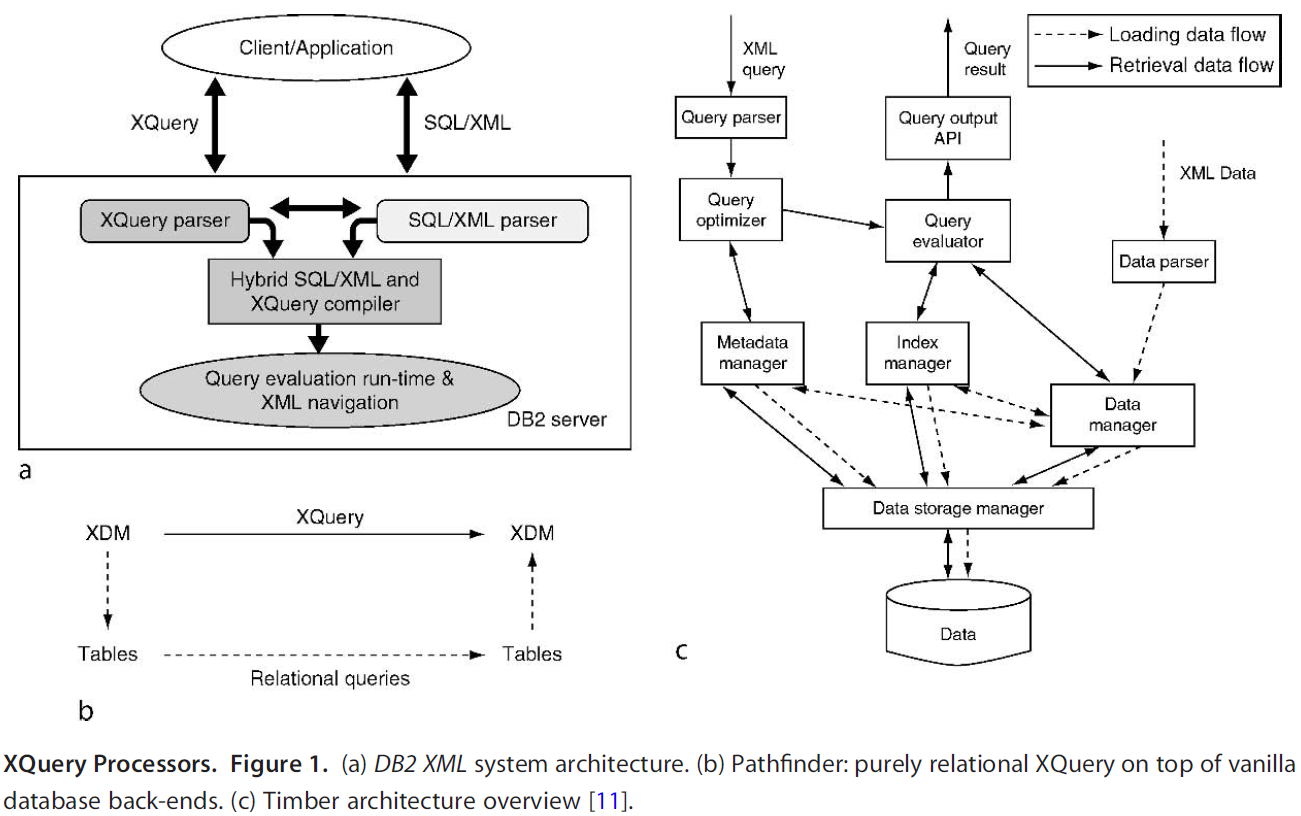
\includegraphics[width=\textwidth,height=0.77\textheight,keepaspectratio]{xml-approaches.png} 
\footnote{\tiny{Изображение взято из \cite{Grust2009}}}
\end{figure}    
  
\end{frame}
\end{comment}

\begin{frame}[allowframebreaks]
\frametitle{Ссылки}
\footnotesize{
\begin{thebibliography}{99}
	
\bibitem[Yianilos, 1993] {Yianilos1993} Peter N. Yianilos. 1993. Data structures and algorithms for nearest neighbor search in general metric spaces. In Proceedings of the fourth annual ACM-SIAM symposium on Discrete algorithms (SODA '93). Society for Industrial and Applied Mathematics, Philadelphia, PA, USA, 311-321. 

\bibitem[Gionis et al., 1999] {Gionis1999} Aristides Gionis, Piotr Indyk, and Rajeev Motwani. 1999. Similarity Search in High Dimensions via Hashing. In Proceedings of the 25th International Conference on Very Large Data Bases (VLDB '99), Malcolm P. Atkinson, Maria E. Orlowska, Patrick Valduriez, Stanley B. Zdonik, and Michael L. Brodie (Eds.). Morgan Kaufmann Publishers Inc., San Francisco, CA, USA, 518--529. 

\bibitem[Ciaccia et al., 1997] {Ciaccia1997} Paolo Ciaccia, Marco Patella, and Pavel Zezula. 1997. M-tree: An Efficient Access Method for Similarity Search in Metric Spaces. In Proceedings of the 23rd International Conference on Very Large Data Bases (VLDB '97), Matthias Jarke, Michael J. Carey, Klaus R. Dittrich, Frederick H. Lochovsky, Pericles Loucopoulos, and Manfred A. Jeusfeld (Eds.). Morgan Kaufmann Publishers Inc., San Francisco, CA, USA, 426--435. 

\bibitem[Qian et al., 2006] {Qian2006} Gang Qian, Qiang Zhu, Qiang Xue, and Sakti Pramanik. 2006. Dynamic indexing for multidimensional non-ordered discrete data spaces using a data-partitioning approach. ACM Trans. Database Syst. 31, 2 (June 2006), 439--484. DOI=http://dx.doi.org/10.1145/1138394.1138395 

\bibitem[Eltabakh et al., 2006] {Eltabakh2006} M. Y. Eltabakh, R. Eltarras and W. G. Aref, "Space-Partitioning Trees in PostgreSQL: Realization and Performance," 22nd International Conference on Data Engineering (ICDE'06), 2006, pp. 100--100. doi: 10.1109/ICDE.2006.146

\bibitem[Papadopoulos et al., 2009] {Papadopoulos2009} Apostolos N. Papadopoulos, Antonio Corral, Alexandros Nanopoulos, Yannis Theodoridis. R-Tree (and Family). Ling Liu, M. Tamer Özsu (Eds.): Encyclopedia of Database Systems. 2453--2459. Springer US 2009, ISBN 978-0-387-35544-3, 978-0-387-39940-9.

\bibitem[Brakatsoulas et al., 2002] {Brakatsoulas2002} Sotiris Brakatsoulas, Dieter Pfoser, and Yannis Theodoridis. 2002. Revisiting R-Tree Construction Principles. In Proceedings of the 6th East European Conference on Advances in Databases and Information Systems (ADBIS '02), Yannis Manolopoulos and Pavol Návrat (Eds.). Springer-Verlag, London, UK, UK, 149--162. 

\bibitem[Grigorev and Chernishev, 2016] {Grigorev2016} Valentin Grigorev and George Chernishev. 2016. K-means Split Revisited: Well-grounded Approach and Experimental Evaluation. In Proceedings of the 2016 International Conference on Management of Data (SIGMOD '16). ACM, New York, NY, USA, 2251--2252. DOI: http://dx.doi.org/10.1145/2882903.2914833 

\bibitem[Manolopoulos et al., 2005] {Manolopoulos2005} Yannis Manolopoulos, Alexandros Nanopoulos, Apostolos N. Papadopoulos, and Yannis Theodoridis. 2005. R-Trees: Theory and Applications. Springer Publishing Company, Incorporated. 

%\bibitem[Mitchel, 1993] {Mitchel1993} Gail Anne Mitchel. Extensible Query Processing in an Object-Oriented Database. Technical Report TR93-16. Department of Computer Science, Brown University. \url{ftp://ftp.cs.brown.edu/pub/techreports/93/cs93-16.pdf}

%\bibitem[Ozsu and Blakeley, 1990] {Ozsu0} M. Tamer Özsu and Jose A. Blakeley. Query Processing in Object-Oriented Database Systems. 19 pages. \url{https://cs.uwaterloo.ca/~tozsu/publications/odbms/wonkim/kimchap.pdf}

%\bibitem[Straube and Ozsu, 1990] {Straube1987} David D. Straube and M. Tamer Özsu. 1990. Queries and query processing in object-oriented database systems. ACM Trans. Inf. Syst. 8, 4 (October 1990), 387--430. DOI=http://dx.doi.org/10.1145/102675.102678 

%\bibitem[Rowe and Stonebraker, 1987] {Rowe1987} Rowe L. and Stonebraker M. The Postgres Data Model. In Proc. 13th Int. Conf. on Very Large Data Bases. 1987.

%\bibitem[Urban and Dietrich, 2009] {Urban2009} Susan D. Urban, Suzanne W. Dietrich. Object Data Models. Encyclopedia of Database Systems. Springer US, 2009. 1929--1935. \url{http://dx.doi.org/10.1007/978-0-387-39940-9_249}

%\bibitem[Jagadish et al., 2002] {Jagadish2002} H. V. Jagadish, S. Al-Khalifa, A. Chapman, L. V. S. Lakshmanan, A. Nierman, S. Paparizos, J. M. Patel, D. Srivastava, N. Wiwatwattana, Y. Wu, and C. Yu. 2002. TIMBER: A native XML database. The VLDB Journal 11, 4 (December 2002), 274--291. DOI=http://dx.doi.org/10.1007/s00778-002-0081-x 

%\bibitem[Luna Dong and Srivastava, 2009] {Luna2009} Xin Luna Dong, Divesh Srivastava. XML Indexing. Encyclopedia of Database Systems. Springer US, 2009. 3585--3591. \url{http://dx.doi.org/10.1007/978-0-387-39940-9_779}

%\bibitem[Grust et al., 2009] {Grust2009} Torsten Grust, H. V. Jagadish, Fatma Ozcan, Cong Yu. XQuery Processors. Encyclopedia of Database Systems. Springer US, 2009. 3671--3675.

%\bibitem[Hidders and Paredaens, 2009] {Hidders2009} Jan Hidders and Jan Paredaens. XPath/XQuery. Encyclopedia of Database Systems. Springer US, 2009. 3659--3665.\url{http://dx.doi.org/10.1007/978-0-387-39940-9_774}

%\bibitem[Taranov et al., 2010] {Taranov2010} Ilya Taranov, Ivan Shcheklein, Alexander Kalinin, Leonid Novak, Sergei Kuznetsov, Roman Pastukhov, Alexander Boldakov, Denis Turdakov, Konstantin Antipin, Andrey Fomichev, Peter Pleshachkov, Pavel Velikhov, Nikolai Zavaritski, Maxim Grinev, Maria Grineva, and Dmitry Lizorkin. 2010. Sedna: native XML database management system (internals overview). In Proceedings of the 2010 ACM SIGMOD International Conference on Management of data (SIGMOD '10). ACM, New York, NY, USA, 1037-1046. DOI=http://dx.doi.org/10.1145/1807167.1807282 

%\bibitem[Ivanova et al., 2010] {Ivanova2010} Milena G. Ivanova, Martin L. Kersten, Niels J. Nes, and Romulo A.P. Gonçalves. 2010. An architecture for recycling intermediates in a column-store. ACM Trans. Database Syst. 35, 4, Article 24 (October 2010), 43 pages. DOI=10.1145/1862919.1862921 http://doi.acm.org/10.1145/1862919.1862921 

%\bibitem[Shatdal et al., 1994] {Shatdal1994} Ambuj Shatdal, Chander Kant, and Jeffrey F. Naughton. 1994. Cache Conscious Algorithms for Relational Query Processing. In Proceedings of the 20th International Conference on Very Large Data Bases (VLDB '94), Jorge B. Bocca, Matthias Jarke, and Carlo Zaniolo (Eds.). Morgan Kaufmann Publishers Inc., San Francisco, CA, USA, 510--521. 

%\bibitem[Boncz et al., 2008] {Boncz2008} Peter A. Boncz, Martin L. Kersten, and Stefan Manegold. 2008. Breaking the memory wall in MonetDB. Commun. ACM 51, 12 (December 2008), 77--85. DOI=http://dx.doi.org/10.1145/1409360.1409380 

%\bibitem[Boncz et al., 2005] {Boncz2005} Peter Boncz, Marcin Zukowski, Niels Nes. MonetDB/X100: Hyper-Pipelining Query Execution. CIDR'05.

%\bibitem[Hennessy and Patterson, 2011] {Hennessy2011}  John L. Hennessy and David A. Patterson. 2011. Computer Architecture, Fifth Edition: A Quantitative Approach (5th ed.). Morgan Kaufmann Publishers Inc., San Francisco, CA, USA. 

%\bibitem[Tsirogiannis et al., 2009] {Tsirogiannis2009}  Dimitris Tsirogiannis, Stavros Harizopoulos, Mehul A. Shah, Janet L. Wiener, and Goetz Graefe. 2009. Query processing techniques for solid state drives. In Proceedings of the 2009 ACM SIGMOD International Conference on Management of data (SIGMOD '09), Carsten Binnig and Benoit Dageville (Eds.). ACM, New York, NY, USA, 59-72. DOI=http://dx.doi.org/10.1145/1559845.1559854 

%\bibitem[Li and Ross, 1999] {Li1999} Zhe Li and Kenneth A. Ross. 1999. Fast joins using join indices. The VLDB Journal 8, 1 (April 1999), 1--24. DOI=http://dx.doi.org/10.1007/s007780050071 

%\bibitem[Star Schema Benchmark Specification, 2009] {SSB} Star Schema Benchmark. Revision 3, June 5, 2009 Pat O'Neil, Betty O'Neil, Xuedong Chen

%\bibitem[Abadi et al., 2008] {Abadi2008} Daniel J. Abadi, Samuel R. Madden, and Nabil Hachem. 2008. Column-stores vs. row-stores: how different are they really?. In Proceedings of the 2008 ACM SIGMOD international conference on Management of data (SIGMOD '08). ACM, New York, NY, USA, 967-980. DOI=http://dx.doi.org/10.1145/1376616.1376712 

%\bibitem[TPC-H Specification, 2011] {TPC-H} TPC BENCHMARK(TM) H (Decision Support) Standard Specification Revision 2.14.2

%\bibitem[Abadi et al., 2012] {Abadi2013} Daniel Abadi, Peter Boncz, Stavros Harizopoulos. The Design and Implementation of Modern Column-Oriented Database Systems. Foundations and Trends(R) in Databases Vol. 5, No. 3 (2012) 197--280

%\bibitem[Harizopoulos et al., 2009] {Harizopoulos2009} Stavros Harizopoulos, Daniel Abadi, Peter Boncz. Column-Oriented Database Systems. VLDB 2009 Tutorial (slides).

% \bibitem[Чернышев, 2013] {Chernishev2013}	Г. А. Чернышев, <<Организация физического уровня колоночных СУБД>>, Тр. СПИИРАН, 30 (2013), 204--222

% \bibitem[Кузнецов, 2010] {Kuznetsov2010}	 Кузнецов С.Д., <<Год эпохи перемен в технологии баз данных>>, Труды Института системного программирования РАН, 19 (2010), 9--34

%\bibitem[Elnikety, 2009] {Elnikety2009} Distributed DBMS. Sameh Elnikety. Encyclopedia of Database Systems. Ling Liu and M. Tamer {\"O}zsu (eds), p. 896--899. Springer US, 2009. \url{http://dx.doi.org/10.1007/978-0-387-39940-9\_654}

%\bibitem[Kian-Lee Tan, 2009] {Kian-Lee2009} Distributed Database Systems. Kian-Lee Tan. Encyclopedia of Database Systems. Ling Liu and M. Tamer {\"O}zsu (eds), p. 894--896. Springer US, 2009. \url{http://dx.doi.org/10.1007/978-0-387-39940-9_701}

%\bibitem[{\"O}zsu and Valduriez, 2011] {Ozsu2011} {\"O}zsu M.T. and Valduriez P. Principles of Distributed Database Systems, 3rd ed. Prentice-Hall, 2011.

%\bibitem[Kossmann, 2000] {Kossmann2000} Donald Kossmann. 2000. The state of the art in distributed query processing. ACM Comput. Surv. 32, 4 (December 2000), 422--469. DOI=http://dx.doi.org/10.1145/371578.371598 


%\bibitem[Ioannidis, 2003] {Ioannidis2003}  Yannis Ioannidis. 2003. The history of histograms (abridged). In Proceedings of the 29th international conference on Very large data bases - Volume 29 (VLDB '03), Johann Christoph Freytag, Peter C. Lockemann, Serge Abiteboul, Michael J. Carey, Patricia G. Selinger, and Andreas Heuer (Eds.), Vol. 29. VLDB Endowment 19--30. 

%\bibitem[Ioannidis and Poosala, 1995] {Ioannidis1995} Y. Ioannidis and V. Poosala. Histogram Based Solutions to Diverse Database Estimation Problems, IEEE Data Engineering, Vol. 18, No. 3, pp. 10--18, September 1995.

%\bibitem[Poosala et al., 1996] {Poosala1996} Viswanath Poosala, Peter J. Haas, Yannis E. Ioannidis, and Eugene J. Shekita. 1996. Improved histograms for selectivity estimation of range predicates. In Proceedings of the 1996 ACM SIGMOD international conference on Management of data (SIGMOD '96), Jennifer Widom (Ed.). ACM, New York, NY, USA, 294--305. DOI=http://dx.doi.org/10.1145/233269.233342 


%\bibitem[Kooi, 1980] {Kooi1980} Robert Philip Kooi. The Optimization of Queries in Relational Databases. PhD Thesis, Case Western Reserve University (1980).

%\bibitem[Piatetsky-Shapiro and Connel, 1984] {Piatetsky-Shapiro1984} Gregory Piatetsky-Shapiro and Charles Connell. 1984. Accurate estimation of the number of tuples satisfying a condition. In Proceedings of the 1984 ACM SIGMOD international conference on Management of data (SIGMOD '84). ACM, New York, NY, USA, 256--276. DOI=http://dx.doi.org/10.1145/602259.602294 


%\bibitem[Garcia-Molina et al., 2004] {Ulman2004} Гектор Гарсиа-Молина, Джеффри Д. Ульман, Дженнифер Уидом. Системы баз данных. Полный курс.  ISBN 5-8459-0384-Х; 2004 г. 

%\bibitem[Hellerstein et al., 2007] {Hellerstein2007} Joseph M. Hellerstein, Michael Stonebraker, and James Hamilton. Architecture of a Database System. Found. Trends databases 1, 2 (February 2007), 141--259. 

%\bibitem[Neumann, 2009] {Neumann2009} Thomas Neumann. Query Optimization (in Relational Databases). Encyclopedia of Database Systems. Springer US, 2009. 2273--2278.\url{http://dx.doi.org/10.1007/978-0-387-39940-9_293}

%\bibitem[Selinger et al., 1979] {Selinger1979} Selinger P.G., Astrahan M.M., Chamberlin D.D., Lorie R.A., and Price T.G. Access path selection in a relational database management System. In Proc. ACM SIGMOD Int. Conf. on Management of Data, 1979, pp. 23--34.

%\bibitem[Haas et al., 1989] {Haas1989} Haas L.M., Freytag J.C., Lohman G.M., and Pirahesh H. Extensible query processing in starburst. In Proc. ACM SIGMOD Int. Conf. on Management of Data, 1989, pp. 377--388.

%\bibitem[Graefe, 1995] {Graefe1995} Graefe G. The cascades framework for query optimization. Q. Bull. IEEE TC on Data Engineering, 18(3):19--29, 1995.

%\bibitem[Graefe and McKenna, 1993] {Graefe1993} Graefe G. and McKenna W.J. The volcano optimizer generator: Extensibility and efficient search. In Proc. 9th Int. Conf. on Data Engineering, 1993, pp. 209--218.

%\bibitem[Chaudhuri, 1998] {Chaudhuri1998} Chaudhuri S. An overview of query optimization in relational systems. In Proc. 17th ACM SIGACT-SIGMOD-SIGART Symp. Principles of Database Systems, 1998, pp. 34--43.

%\bibitem[Ioannidis, 1996] {Ioannidis1996} Ioannidis Y. Query optimization. In Handbook of Computer Science, A.B. Tucker (ed.). CRC Press, 1996.

%\bibitem[Jarke and Koch, 1984] {Chaudhuri1984} Jarke M. and Koch J. Query optimization in database systems. ACM Comput. Surv., 16(2):111–152, 1984.

%\bibitem[Ioannidis, 1996] {Ioannidis1996} Yannis E. Ioannidis. 1996. Query optimization. ACM Comput. Surv. 28, 1 (March 1996), 121--123. DOI=http://dx.doi.org/10.1145/234313.234367 

%\bibitem[Graefe, 1996] {Graefe1996} Goetz Graefe. 1996. Iterators, schedulers, and distributed-memory parallelism. Softw. Pract. Exper. 26, 4 (April 1996), 427--452. DOI=http://dx.doi.org/10.1002/(SICI)1097-024X(199604)26:4<427::AID-SPE20>3.3.CO;2-8 

%\bibitem[Taniar et al., 2008] {Taniar2008} David Taniar, Clement H. C. Leung, Wenny Rahayu, and Sushant Goel. 2008. High Performance Parallel Database Processing and Grid Databases. Wiley Publishing. 

%\bibitem[Ramakrishnan and Gehrke, 2000] {Ramakrishnan2000}  Raghu Ramakrishnan and Johannes Gehrke. 2000. Database Management Systems (2nd ed.). Osborne/McGraw-Hill, Berkeley, CA, USA. 

\end{thebibliography}
}
\end{frame}


\end{document} 